
\chapter{Relation to Experimental Data}
\label{chap:exp}

%%%%%%%%%\footnote{A nice and intuitive discusion of the concept of quasiarticle can be found in Chapter 0 of R. D. Mattuck, {\em A Guide to Feynmnan Diagrams in the Many-Body Problem}, McGraw-Hill (1976) [reprinted by Dover].}


In this chapter we will partially explore the connection between the information 
contained in various propagators and experimental data.
The focus is on the experimental properties that are
probed by the removal of particles.
Also, from now on, we will only consider fermionic systems.


An important case is when the spectrum for the $N \pm 1$-particle
system near the Fermi energy involves discrete bound states. This 
happens in finite system like nuclei or molecules.
%
In these cases the main quantity of interest is the overlap wave function, which appears in the
residues of Eq.~(\ref{g1w_Leh}) and in Eq.~(\ref{S1h_ab}). This is
\begin{eqnarray}
\psi^{overlap}_k({\bf r}) &=& \bra{\Psi^{N-1}_k} \psi_s({\bf r}) \ket{\Psi^N_0}
\nonumber \\
 &=& \sqrt{N} \int d{\bf r}_2 \int d{\bf r}_3 \cdots \int d{\bf r}_N
 \label{overlap} \\
&& \qquad  \times [ \Psi^{N-1}_k({\bf r}_2, {\bf r}_3, \ldots {\bf r}_N) ]^*
     \Psi^N_0({\bf r}, {\bf r}_2, {\bf r}_3, \ldots {\bf r}_N) \; .
\nonumber
\end{eqnarray}
The second line in Eq.~(\ref{overlap}) can be proved by using relations~(\ref{rN_state}) and~(\ref{PhiN_wf}).
This integral comes out in the description of most particle knock out processes because it represents the matrix element between the initial and final states, in the case when the emitted particle is ejected with energy large enough the it interacts only weakly with the residual system.
The quantity of interest here is the so called spectroscopic factor to the final state $k$,
\begin{equation}
S_k = \int d{\bf r} \vert \psi^{overlap}_k({\bf r}) \vert^2 \; .
\label{SF}
\end{equation}
When the system is made of completely non interacting particles, $S_k$ is unity. In real cases however, correlations among the constituents reduce this value. The possibility of extracting this quantity from experimental data gives us information on the spectral function and therefore on the structure of the correlated system.
% Useful information is also extracted from the shape of the 




\subsection{Spectroscopic strength from particle emission}

In order to make the connection with experimental data obtained from
knockout reactions, it is useful to consider the response of a system to a weak
probe. The hole spectral function introduced in Eq.~(\ref{S1h_ab}) can be 
substantially ``observed'' these reactions. The general 
idea is to transfer a large amount of momentum and energy to a 
particle of a bound system in the ground state.
This is then ejected from 
the system, and one ends up with a fast-moving particle and a bound 
$(N-1)$-particle system. By observing the momentum of the ejected 
particle it is then possible the reconstruct the spectral function of the 
system, provided that the interaction between the ejected particle and the 
remainder is sufficiently weak or treated in a controlled fashion,
\textit{e. g.} by constraining this treatment with information from other
experimental data.  

We assume that the  $N$-particle system is initially in its ground 
state,
\begin{equation}
\ket{\Psi_i} =\ket{\Psi^N_0 },
\end{equation}
and makes a transition to a final $N$-particle eigenstate 
\begin{equation}
\label{dim:eep1}
\ket{\Psi_f}= a^{\dagger}_{\bm p}\ket{\Psi^{N-1}_{n}},
\end{equation}
composed of a bound $(N-1)$-particle eigenstate, 
$\ket{\Psi^{N-1}_{n}}$, and a particle with momentum $\bm{p}$.

For simplicity we consider the transition matrix elements for a scalar 
external probe 
\begin{equation}
\rho ({\bm q})=\sum_{j=1}^N \exp{(i{\bm q}\cdot{\bm r}_j)},
\label{eq:eep0}
\end{equation} 
which transfers momentum $\bm{q}$ to a particle.   
Suppressing other possible sp quantum numbers, like $\textit{e.g.}$ spin,
the second-quantized form of this operator is given by
\begin{equation} 
\hat{\rho}({\bm q}) = \sum_{\bm{p},\bm{p}'}\bra{\bm{p}}\exp{(i{\bm q}
\cdot{\bm r})}\ket{\bm{p}'}a^{\dagger}_{\bm p}a_{\bm{p}'}
=\sum_{\bm p} a^{\dagger}_{\bm p} a_{{\bm p}-{\bm q}}.
\end{equation}
The transition matrix element now becomes 
\begin{eqnarray}
\bra{\Psi_f }\hat{\rho}({\bm q})\ket{\Psi_i }&=&
\sum_{\bm{p}'} \bra{\Psi^{N-1}_{n}}a_{\bm{p}} a^{\dagger}_{\bm{p}'}
a_{\bm{p}'-\bm{q}}\ket{\Psi^N_0}
\nonumber \\
&=&
\sum_{\bm{p}'} \bra{\Psi^{N-1}_{n}}\delta_{\bm{p}',\bm{p}}
a_{\bm{p}'-\bm{q}}
+a^{\dagger}_{\bm{p}'}a_{\bm{p}'-\bm{q}}a_{\bm p} \ket{\Psi^N_0 }
\nonumber\\ 
&\approx
&\bra{\Psi^{N-1}_{n}}a_{{\bm p}-{\bm q}}\ket{\Psi^N_0 } .
\label{dim:eep2}
\end{eqnarray}
The last line is obtained in the so-called {\em Impulse Approximation} (or {\em Sudden Approximation}), 
where it is assumed that the ejected particle is the one that has absorbed 
the momentum from the external field. This is a very good approximation 
whenever the momentum ${\bm p}$ of the ejectile is much larger than typical 
momenta for the particles in the bound states; the neglected term in 
Eq.~(\ref{dim:eep2}) is then very small, as it involves the removal of a 
particle with momentum  ${\bm p}$ from $\ket{\Psi^N_0}$. 

There is one other assumption in 
the derivation: the fact that the final eigenstate of the $N$-particle system 
was written in the form of Eq.~(\ref{dim:eep1}), 
i.e.\ a plane-wave state for the ejectile on top of an $(N-1)$-particle 
eigenstate. This is again a good approximation 
if the ejectile momentum is large enough, as can be understood by rewriting 
the Hamiltonian in the $N$-particle system as 
\begin{equation} 
\label{dim:eep3}
H_N=\sum_{i=1}^N \frac{{\bm p}^2_i}{2m}+\sum_{i<j=1}^N V(i,j) 
=H_{N-1}+\frac{{\bm p}^2_N}{2m}+\sum_{i=1}^{N-1} V(i,N) .
\end{equation}
The last term in Eq.~(\ref{dim:eep3}) represents the 
{\em Final State Interaction}, or the 
interaction between the ejected particle $N$ and the other 
particles $1\dots N-1$. If the relative momentum between particle $N$ and the 
others is large enough their mutual interaction can be neglected, and 
$H_N \approx H_{N-1} + \bm{p}^2_N/2m$. 
The result given by Eq.~(\ref{dim:eep2}) is called the 
{\em Plane Wave Impulse Approximation} or 
PWIA knock-out amplitude, for obvious reasons, and is precisely 
a removal amplitude (in the momentum representation) appearing in the Lehmann
representation of the sp propagator [Eq.~(\ref{overlap}) and~(\ref{S1h_ab})].

The cross section of the knock-out reaction, where the momentum and energy of
the ejected particle and the probe are either measured or known, is according 
to Fermi's golden rule proportional to
\begin{equation}
\label{dim:eep4}
d\sigma \sim
\sum_n \delta (\omega 
+E_i -E_f) |\bra{\Psi_f}\hat{\rho}({\bm q})\ket{\Psi_i}|^2,
\end{equation}
where the energy-conserving $\delta$-function contains the energy transfer 
$\omega$ of the probe, and the initial and final energies of the system 
are $E_i = E^N_0$ and $E_f =E^{N-1}_n +{\bm p}^2/2m$, respectively. Note that 
the internal state of the residual $N-1$ system is not measured, hence the 
summation over $n$ in Eq.~(\ref{dim:eep4}). 
Defining the missing momentum $\bm{p}_{miss}$ and missing energy $E_{miss}$ 
of the 
knock-out reaction as\footnote{We will neglect here the recoil of the residual
$N-1$ system, i.e.\ we assume the mass of the $N$ and $N-1$ system to be much 
heavier than the mass $m$ of the ejected particle.}
\begin{equation}
\bm{p}_{miss}={\bm p} - {\bm q}
\label{eq:eepx}
\end{equation}
and
\begin{equation}
E_{miss} ={\bm p}^2/2m -  \omega = E^N_0-E^{N-1}_n ,
\label{eq:eepy}
\end{equation} 
respectively,
the PWIA knock-out cross section can be rewritten as 
\begin{eqnarray} 
d\sigma &\sim&
\sum_n \delta (E_{miss}-E^N_0+E^{N-1}_n ) |\bra{\Psi^{N-1}_{n}}
a_{\bm{p}_{miss}}\ket{\Psi^N_0 }|^2
\nonumber\\
& = & S^h (\bm{p}_{miss},E_{miss}) .
\label{dim:eep6}
\end{eqnarray}
The PWIA cross section is therefore exactly proportional to the diagonal
part of the hole spectral function defined in Eq.~(\ref{S1h_ab}). 
This is of course only true in the PWIA, but when the 
deviations of the impulse approximation and the effects of the final state 
interaction are under control, it is possible to obtain precise 
experimental information on the hole spectral function of the system under 
study.



\subsection{An example: the $(e,e'p)$ reaction}

Several studies of reacton theory have been done in past years
constrain and improve the analysis of electron scattering reactions\footnote{See for example, 
S.~Boffi, C.~Giusti, F.~D.~Pacati, and M.~Radici,
{\em Electromagnetic Response of Atomic nuclei}, 
Oxford Studies in Nuclear Physics (Clarendon, Oxford, 1996).}.
 Although the actual (e,e$'$p) experiments involve more complicated
one-body excitation operators than the one considered in the simple simple
example above, the basic conclusions are not altered%
\footnote{S. Frullani and J. Mougey, Adv. Nucl. Phys. \textbf{14}, 1 (1984).}.



%An even more realistic description of the proton knockout reaction
%again identifies the external electron probe and the corresponding
%virtual photon as represented by a one-body excitation operator.
%\begin{equation}
%\hat{O} = \sum_{\alpha \beta} \bra{\alpha} O \ket{\beta} a^\dagger_\alpha
%a_\beta .
%\label{eq:op}
%\end{equation}
%The response of the system to such an external excitation operator is described
%by the polarization propagator which has a Lehmann representation
%given by Eq.~(\ref{eq:Pi_Leh}).
%The transition probability induced by $\hat{O}$
%from the ground state to an excited state is given by
%\begin{equation}
%\left| \bra{\Psi^A_n} \hat{O} \ket{\Psi^A_0} \right|^2 =
%\sum_{\alpha \beta} \sum_{\gamma \delta} 
% \bra{\gamma} O \ket{\delta} \bra{\Psi^A_n} a^\dagger_\gamma 
%a_\delta \ket{\Psi^A_0} 
% \bra{\alpha} O \ket{\beta}^* \bra{\Psi^A_n} a^\dagger_\alpha 
%a_\beta \ket{\Psi^A_0}^* .
%\label{eq:14.6}
%\end{equation}
%This result demonstrates that the numerator of the first term in
%Eq.~(\ref{eq:Pi_Leh}) contains the relevant transition amplitudes for a
%given state $n$ to evaluate this transition probability.
%In general, there are important correlations between the ph states,
%in particular at low energy where collective surface vibrations and
%giant resonances occur.
%At higher excitation energy and momentum transfer, these collective
%coherence effects tend to disappear.
%In this domain, one may therefore write the polarization propagator
%as the product of two dressed sp propagators as in Eq.~(\ref{eq:Pif}).
%Replacing $\Pi$ by this dressed $\Pi^{f}$ one neglects contributions
%where the particle and hole interact but includes all other correlations
%associated with the full dressing of the removed particle in terms
%of the corresponding removal amplitude (or spectral function) and
%the corresponding dressing of the particle that will ultimately be detected
%in the (e,e$'$p) experiment.
%The wave function of this dressed particle corresponds to the addition
%amplitude in coordinate space and can be associated with an optical model
%wave function~\cite{masa91}.
%
%From this analysis it becomes therefore clear that one may use empirical
%information associated with the elastic scattering of protons in terms
%of optical potentials to describe this wave function of the outgoing
%proton.
%Clearly, it is this interpretation that clarifies the assumptions that
%underly the standard analyis of the (e,e$'$p) reaction~\cite{deWitt1} - 
%\cite{Paviabook}.%
%


In the practical analysis of an (e,e$'$p) experiment it is conventional to find
a local potential well (mostly of Woods-Saxon type) which will generate a sp
state at the removal energy for the transition that is studied.
This state is further required to provide the best possible fit to
the experimental momentum dependence of the cross section (with proper
inclusion of complications due to electron and proton 
distortion).
The overall factor necessary to bring the resulting calculated cross section
into agreement with the experimental data, can then be interpreted as the
spectroscopic factor corresponding to the ``experimental''
quasihole wave function
according to Eq.(\ref{SF}).



The resulting cross sections obtained at 
the NIKHEF facility are shown for four different nuclei
in Fig.~\ref{fig:louk1}%
\footnote{L. Lapik\'{a}s, Nucl. Phys. {\bf A553}, 297c (1993).}
\begin{figure}[tbb]
  \begin{center}
    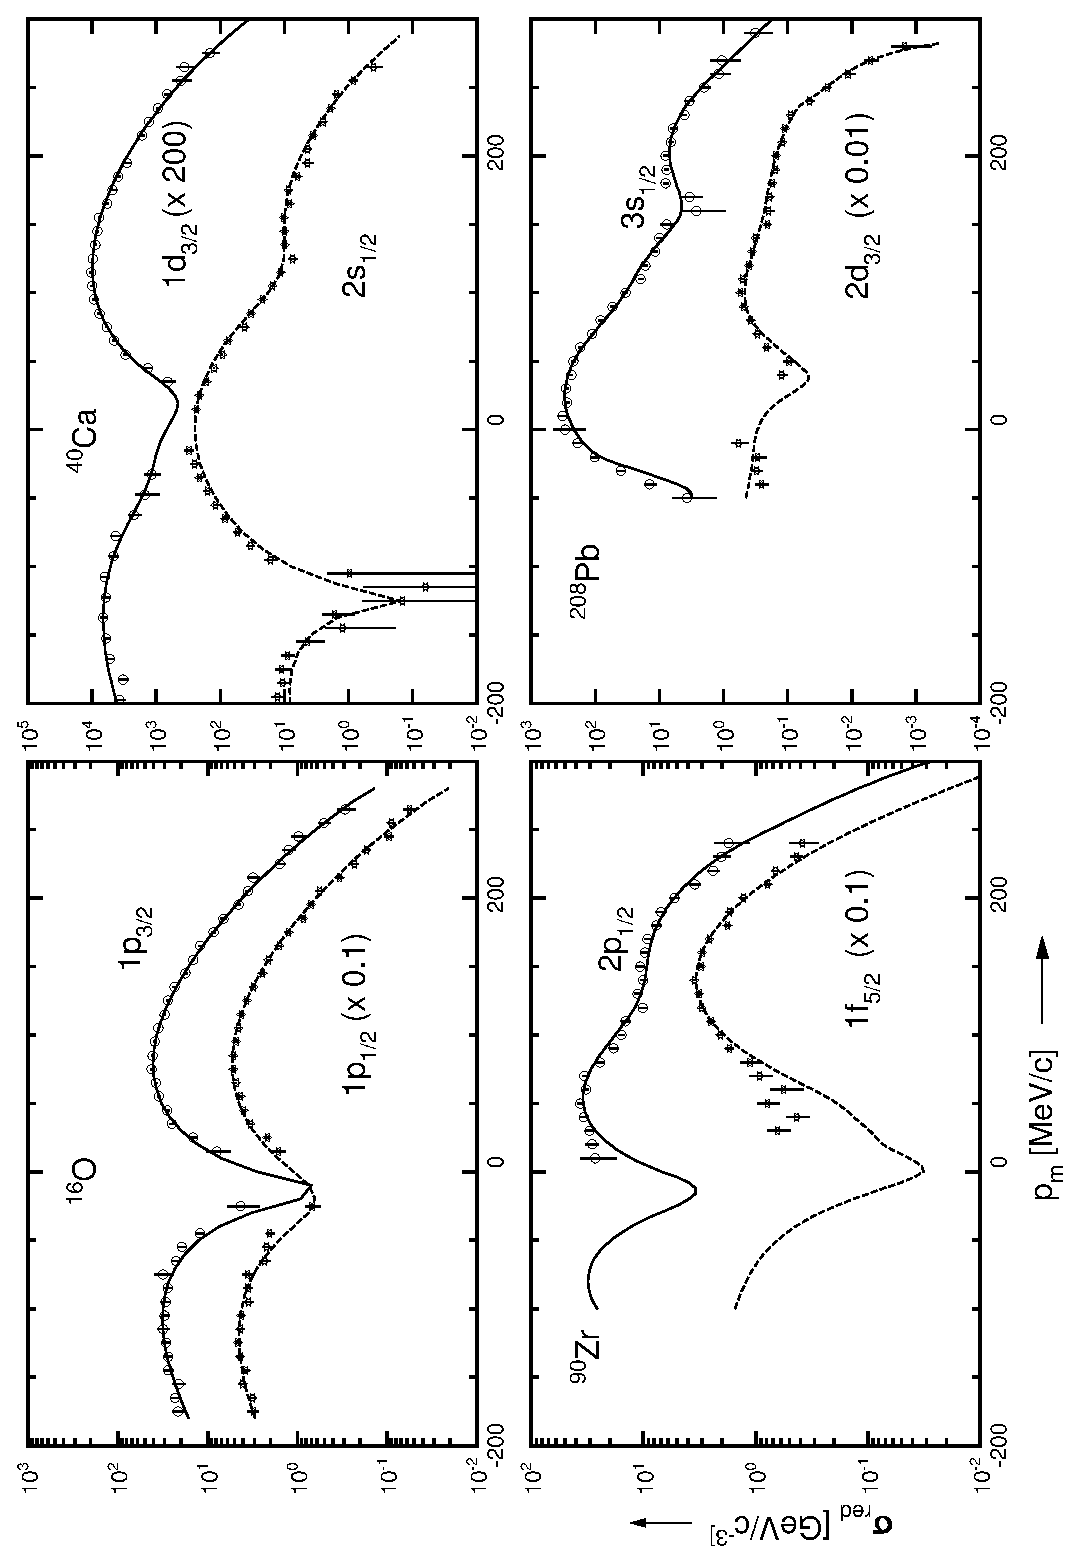
\includegraphics[height=0.65\textheight,angle=-90]{plotprlands.eps}
    \end{center}
    \caption{\label{fig:louk1}
      Momentum distributions for various nuclei obtained from the
(e,e$'$p)\ reaction performed at NIKHEF~(Note n. 4, p. 28).}
\end{figure}
It is important to realize that the shapes of the wave functions
in momentum space correspond closely to the ones expected on
the basis of a standard Woods-Saxon potential well (or more involved
mf wave functions).
This is itself an important observation since the (e,e$'$p) reaction
probes the interior of the nucleus, a feat not available with hadronically
induced reactions.

While the shapes of the valence nucleon wave functions correspond to the basic
ingredients expected on the basis of years of nuclear structure physics
experience, there is a significant departure with regard to the integral
of the square of these wave functions.
This quantity is of course the spectroscopic factor
and is shown in Fig.~\ref{fig:louk2} for the data obtained at 
NIKHEF.
\begin{figure}[!pbt]
\vspace*{.5cm}       
 \begin{center}
    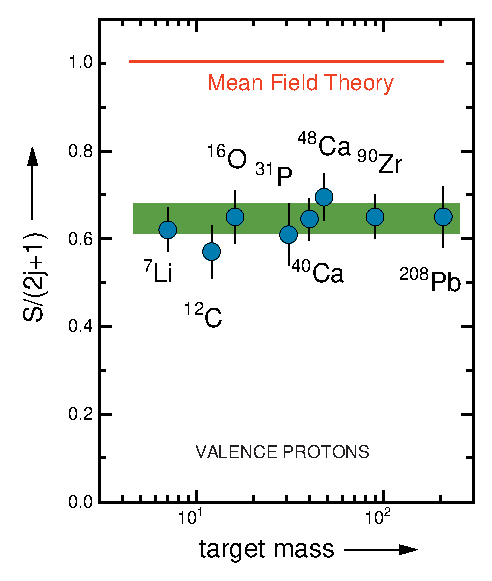
\includegraphics[height=0.30\textheight]{saval2c.eps}
\end{center}
\caption{Spectroscopic factors from the (e,e$'$p) reaction as a function
of target mass. Data have been obtained at the NIKHEF facility~(Note n. 4, p. 28).
\label{fig:louk2} }
\end{figure}
The results shown in Fig.~\ref{fig:louk2} indicate that there is an
essentially global reduction of the sp strength of about
35 \% 
which needs to be explained by the theoretical calculations.
This depletion is somewhat less for the strength associated with slightly
more bound levels.
An additional feature obtained in the (e,e$'$p) reaction is the fragmentation
pattern of these more deeply bound orbitals in nuclei.
This pattern is such that single isolated peaks are obtained only
in the immediate vicinity
of the Fermi energy whereas for more deeply bound states a stronger
fragmentation of the strength is obtained with larger distance from
$\varepsilon_F$.
This is beautifully illustrated by the (e,e$'$p)\ data from 
Quint\footnote{E. N. M. Quint, Ph.D. thesis, University of Amsterdam (1988).}.
Whereas the $3s_{1/2}$ orbit exhibits a single peak, there is a
substantial fragmentation of the $1f$ strength as indicated in 
this figure.
Additional information about the occupation number of the former orbit 
is also available and can be 
obtained by analyzing elastic electron scattering cross sections of 
neighboring nuclei.
The actual occupation number for the $3s_{1/2}$ proton orbit obtained
from this analysis is about 10\% 
larger than the quasihole spectroscopic
factor~\footnote{P. Grabmayr \textit{et al.}, Phys. Lett. {\bf B164}, 15 (1985). 
P. Grabmayr, Prog. Part. Nucl. Phys. {\bf 29}, 251 (1992).} and therefore corresponds to 0.75.
All these features of the strength need to be explained theoretically.
This will be attempted in the material covered in later sections.


%
%\subsection{Information from the (e,e$'$2N) reaction}
%
%Suggestions to explore SRC in two-nucleon emission
%reactions go back to the work of Gottfried~\cite{GO58}.
%More recently, theoretical work has focused on the possibility to utilize
%the (e,e$'$2N) reaction to probe nucleon-nucleon
%correlations~\cite{CI90} - \cite{BO90}.
%Practical descriptions of this reaction have been developed by 
%the Pavia group~\cite{GP91} - \cite{GP95}.
%Proceeding in a similar vein as in the analysis of the (e,e$'$p) reaction,
%which yields information about the one-nucleon (removal) spectral function, 
%one may hope to learn about the two-nucleon (removal) spectral function
%in two-nucleon emission processes.
%The emission of two protons is particularly promising for studies of
%SRC since the effect of meson-exchange currents and
%isobars is not expected to dominate the cross section
%under suitable kinematic conditions~\cite{GP92}.
%
%Experiments have been carried out for $^{12}$C~\cite{KHK95} and
%$^{16}$O (discussed in more detail in Sec.~\ref{sec:ee1-2N}) 
%to explore the feasibility of gaining insight 
%into nucleon-nucleon correlations in finite nuclei using the (e,e$'$pp)
%reaction. 
%Triple coincidence measurements involving protons with large initial
%momenta seem particularly suitable to provide information on SRC. 
%The scattered electron is then expected to 
%transfer a virtual photon to one of these two protons which have large
%and opposite momenta and therefore a relatively small center-of-mass momentum.
%This strong correlation results from hard collisions due to the strong 
%repulsive core of the NN interaction.
%When one of the protons is removed by the absorption of the virtual photon,
%its partner will also leave the nucleus under the assumption that the 
%energy transfer is mainly to the hit pair (the residual nucleus stays at a 
%low excitation energy)~\cite{GP91}.
%It is therefore hoped that, if the coupling of the virtual photon to one
%nucleon is the dominant mechanism, the
%(e,e$'$pp) process may be exploited as a useful tool to
%investigate these short-range correlation effects (see also Ref.~\cite{Ry94}).
%
%One of the goals of triple coincidence measurements is to illuminate
%the features of the interaction between two nucleons before their knockout
%of the nucleus and their subsequent detection.
%Early experiments on $^{12}$C employing the (e,e$'$pp) reaction
%already assumed in the analysis of the data obtained at 
%NIKHEF~\cite{Kes93,GP91}
%that the virtual photon is coupled to
%one of the detected protons. 
%This approximation can be understood by considering the transition matrix
%element of the nuclear charge operator in momentum space
%	\begin{equation}
%		\hat{\rho} (\bm{q}) = e \sum_{\bm{ p}'} 
%		a^\dagger_{\bm{p}'+\bm{ q}} a_{\bm{p}'} 
%	\label{eq:rhoq}
%	\end{equation}
%%
%(with spin implicit in the summation)
%between the initial state $\ket{\Psi^A_0}$ and an approximate
%final state of the form
%%
%	\begin{equation}
%	\ket{\Psi_{final} } =
%a^\dagger_{\bm{p}_{1'}} a^\dagger_{\bm{p}_{2'}} | \Psi^{A-2}_n \rangle .
%	\label{eq:finst}
%	\end{equation}
%%
%This final state contains two plane wave protons and an exact
%state $\ket{\Psi_n^{A-2}}$ for the system with two protons removed. 
%In calculating the matrix elements of the transition charge operator
%one obtains
%%
%	\begin{equation}
%	\langle \Psi_{final} | {\hat \rho} (\bm{q}) | \Psi^A_0 \rangle =
%\langle \Psi^{A-2}_n | a_{\bm{p}'_2} a_{\bm{p}'_1-\bm{q}}
%| \Psi^A_0 \rangle + \langle \Psi^{A-2}_n |
%a_{\bm{p}'_2-\bm{q}} a_{\bm{p}'_1}| \Psi^A_0 \rangle ,
%	\label{eq:finstme}
%	\end{equation}
%%
%assuming that one of the detected protons absorbs the momentum $\bm{q}$.
%To obtain the contribution to the cross section one requires the square of
%this matrix element.
%This yields four terms, each representing a particular term of 
%Eq.~(\ref{eq:SpecFunc}) for the two-nucleon spectral function.
%An important ingredient in the description of the two-nucleon knock-out 
%reaction is the two-hole spectral function defined by
%	\begin{equation}
%		S^{hh}(\bm{p}_1, \bm{p}_2, \bm{p}_{1'}, \bm{p}_{2'}, 
%		\omega )
%	= \sum_n
%\langle\Psi^A_0| a^\dagger_{\bm{p}_{1'}} a^\dagger_{\bm{p}_{2'}}|%
%		\Psi^{A-2}_n \rangle
%		\langle\Psi^{A-2}_n | a_{\bm{p}_1} a_{\bm{p}_2}|%
%		\Psi^A_0 \rangle
%		\delta( \omega - (E^{A}_0 - E^{A-2}_n) )
%	\;,
%	\label{eq:SpecFunc}
%	\end{equation}
%%
%where $\ket{\Psi^A_0}$ may denote
% the ($0^+$) ground state of the target system 
%(for example $^{16}$O) and $\ket{\Psi^{A-2}_n}$ the $n$-th excited state
%of the residual nucleus ($^{14}$C).
%In Eq.\ (\ref{eq:SpecFunc}), 
% $a^\dagger_{{\bf p}}$ ($a_{{\bf p}}$) represent the addition (removal)
%operators of a nucleon with momentum ${\bf p}$ (spin and isospin are implicit).
%It is therefore clear that the appropriate expression
%for the transition probability is to consider the quantity
%%
%	\begin{eqnarray}
%		\hat{S}(\bm{p}'_1, \bm{p}'_2, E)
%& = &
%		 S^{hh}( \bm{p}'_1-\bm{q}, \bm{p}'_2, 
%		    \bm{p}'_1-\bm{q}, \bm{p}'_2, E )
%		+S^{hh}( \bm{p}'_1-\bm{q}, \bm{p}'_2, 
%		    \bm{p}'_1, \bm{p}'_2-\bm{q}, E )
%	\nonumber \\
%	&+&
%		 S^{hh}( \bm{p}'_1, \bm{p}'_2-\bm{q}, 
%		    \bm{p}'_1-\bm{q}, \bm{p}'_2, E )
%		+S^{hh}( \bm{p}'_1, \bm{p}'_2-\bm{q}, 
%		    \bm{p}'_1, \bm{p}'_2-\bm{q}, E ) 	\;,
%\label{eq:Shat}	
%\end{eqnarray}
%where the vector $\bm{q}$ is the momentum of the virtual photon. 
%
%More realistic implementations of this reaction model naturally require
%the consideration of the distortion effects of the outgoing particles.
%Nevertheless, this simple representation of the reaction clarifies
%the intrinsic importance of two-nucleon spectral functions in
%describing two-nucleon knockout reactions.
%More details related to actual comparison of calculations with
%experimental data will be presented in Sec.~\ref{sec:ee1-2N}.
%%%%%%%%%%%%%%%%%%%%%%%%
